\section*{Appendix A}

\addcontentsline{toc}{section}{Appendix A}

In this section, we provide a proof to Cover's theorem, which deduces storage capacity using the argument that a training set of patterns must be linearly separable for a neural network to be able to store all of the patterns.

Suppose that we have $p$ points in $\mathbb{R}^N$. There are $2^p$ possible partitions of these $p$ points into two classes, for example colouring each point in red or blue. We call a partition that yields linearly separable classes, i.e. where the red and blue points can be separated by a $(N-1)$-dimensional hyperplane a dichotomy. We are interested in determining how many partitions of the $p$ points yield dichotomies.

We assume that the points are in general position, so that any subset of $N$ or fewer points is linearly independent.

Let us denote the number of dichotomies by $C(p, N)$. Suppose that we have $p$ linearly separable points and add a new point P. There are two possibilities of where P can be placed:

\begin{enumerate}
    \item There is a separating hyperplane for the previous $p$ points passing through P. This means that each of the dichotomies for the previous $p$ points yields two distinct dichotomies, because the hyperplane passing through P can be shifted infinitesimally to either side to change the colour of P, without affecting the colourings of any of the previous $p$ points.
    \item There is no separating hyperplane passing through P. The new point P can only have one colour for it to yield a dichotomy, so there is only one new dichotomy for each of the previous dichotomies.
\end{enumerate}

The first case corresponds to $C(p, N-1)$ dichotomies. This is because we take the same $p$ points as before and restrict the dichotomies to those that allow for a separating hyperplane to pass through a point P, which is analogous to restricting the hyperplanes to $N-1$ dimensions instead of $N$, as we can see in Fig. 5.

Thus, to calculate $C(p+1, N)$, we count the number of dichotomies in (1) twice and the number of dichotomies in (2) once. Clearly, this is the same as counting $C(p, N)$ and adding the number of dichotomies in (1).

We can write $C(p, N) = a + b$, where $a$ corresponds to the number of dichotomies in (1) and $b$ corresponds to the number of dichotomies in (2) [\citen{orhanemail}]. Thus, we have:

\begin{align}
    C(p+1, N) & = 2a + b \nonumber \\
    & = a + (a + b) \nonumber \\
    & = C(p, N-1) + C(p, N)
\end{align}

Thus, we have obtained a recurrence equation to find the number of dichotomies in function of the number of points $p$ and input-dimension $N$.

We will now deduce the numerical value of $C(p, N)$ from the recurrence equation. First, we admit that $C(1, k) = 0$ if $k < 1$. We also acknowledge that $C(1, k) = 2$ for $k \geqslant 1$, because a single point can only have two dichotomies in any number of dimensions -- one where the point is coloured red, and one where it is coloured blue.

\pagebreak

\begin{figure}[bhtp]
    \centering
    \captionsetup{justification=centering, font=small, margin=0.5cm}
    \frame{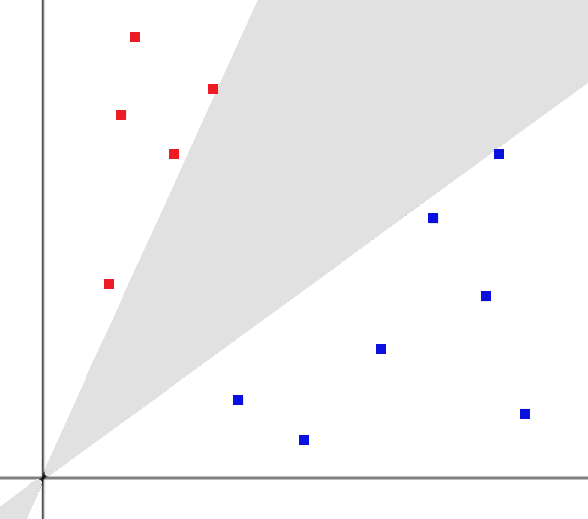
\includegraphics[height=0.25\textwidth]{images/cover-2d-example.png}}
    \caption{For $N=2$, $p=12$, we see that if a new point falls in the shaded area (case 1), it can be coloured either red or blue to create a dichotomy. If the point falls in either of the unshaded areas (case 2), it can only be one of two colours for a dichotomy to exist.}
\end{figure}

\begin{figure}[bhtp]
    \centering
    \captionsetup{justification=centering, font=small, margin=0.5cm}
    \frame{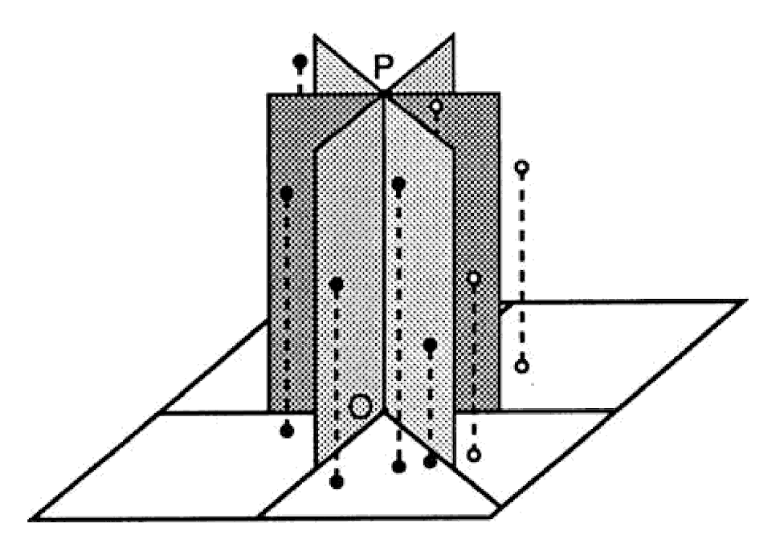
\includegraphics[height=0.25\textwidth]{images/reduce-dimension.png}}
    \caption{Limiting hyperplanes to those that pass through O and P is equivalent to projecting onto the plane perpendicular to OP, thus reducing the dimension of each hyperplane by one. \cite[p.113]{introbook}}
\end{figure}

We observe $p-1$ iterations of (18):

\begin{equation}
    \begin{split}
    C(p+1, N)
    & = C(p, N) + C(p, N-1) \\
    & = C(p-1, N) + 2 C(p-1, N-1) + C(p-1, N-2) \\
    & = \quad ... \\
    & = \binom{p}{0} C(1, N) + \binom{p}{1} C(1, N-1) + ... + \binom{p}{p} C(1, N-p) \end{split}
\end{equation}

From the above observations, we obtain the following hypothesis:

\begin{equation}
    C(p, N) = 2 \sum_{i=0}^{N-1} \binom{p-1}{i}
\end{equation}

By a verification using a proof by induction, we confirm that (20) indeed describes the number of dichotomies in function of the input dimension $N$ and the number of points $p$.

In Fig. 6, we plot the values of $p/N$ against $C(p, N)/2^p$ to see what fraction of partitions of $p$ points a simple perceptron is able to find dichotomies for. We can clearly see that there is a sharp transition with large $N$ when $p = 2N$. At this point, the simple perceptron goes from being able to store all $p$ points to none of them. By definition, this gives the information storage capacity $p_{\max}$ of a simple perceptron:

\begin{equation}
    p_{\max} = 2N
\end{equation}

\pagebreak

\begin{figure}[thbp]
    \centering
    \captionsetup{justification=centering, font=small, margin=0.5cm}
    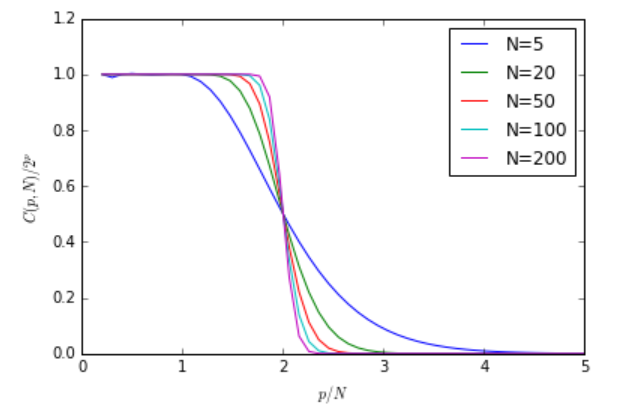
\includegraphics[height=5cm]{images/capacity-graph.png}
    \caption{Fraction of partitions of $p$ points that a perceptron is able to dichotomize for varying values of $N$}
\end{figure}
